% Created 2022-02-22 mar 18:06
% Intended LaTeX compiler: pdflatex
\documentclass[conference]{IEEEtran}
\usepackage[utf8]{inputenc}
\usepackage[T1]{fontenc}
\usepackage{graphicx}
\usepackage{longtable}
\usepackage{wrapfig}
\usepackage{rotating}
\usepackage[normalem]{ulem}
\usepackage{amsmath}
\usepackage{amssymb}
\usepackage{capt-of}
\usepackage{hyperref}
\input{~/org/latex/author_TeoCir2_Riedinger.tex}
\input{~/org/latex/ieee.tex}
\date{\today}
\title{Sistema de adquisión y transmisión de datos autosuficiente y controlable}
\hypersetup{
 pdfauthor={},
 pdftitle={Sistema de adquisión y transmisión de datos autosuficiente y controlable},
 pdfkeywords={},
 pdfsubject={},
 pdfcreator={Emacs 27.2 (Org mode 9.6)}, 
 pdflang={Spanish}}
\begin{document}

\maketitle
\tableofcontents


\section{Descripcion general:}
\label{sec:orgfd88c17}
\subsection{Introduccion:}
\label{sec:orgbe44fea}
El objetivo del proyecto es construir un sistema digital de sensado autosuficiente, con la premisa de ser controlado a través de una estación de recepción de datos.

Esto es, el proyecto se divide en dos sistemas que trabajan de forma codependiente pero que son controlados por microcontroladores distintos:

\begin{itemize}
\item Uno es el \textbf{SATDAC} (Sistema de Adquisicón y Transmisión de Datos Autosuficiente y Controlable), encargado de tomar y procesar muestras u obtener datos.
\item Otro es la \textbf{ERDYTC} (Estación de Recepción de Datos Y Transmisión de Comandos), que se encontraría conectada al SATDAC y se encargaría de mostrar los datos obtenidos.
\end{itemize}

El SATDAC posee las siguientes capacidades:

\begin{itemize}
\item Sensado de variables analógicas; actualmente solo temperatura con presición de 2 decimales en un rango de 22.0 °C a 32 °C.
\item Control y despliegue de periféricos por comando.
\item Almacenamiento en memoria externa.
\item Recepción y transmisión de datos por puerto USART.
\end{itemize}

Físicamente, el SATDAC cuenta con una compuerta que está inicialmente cerrada pero puede ser abierta remotamente solo a través de la ERDYTC.

Y la ERDYTC las siguientes:

\begin{itemize}
\item Capacidad para mostrar datos recibidos y estados en LCD.
\item Ingreso de comandos por usuario y transmisión de los mismos.
\item Recepción y transmisión de datos por puerto USART.
\end{itemize}
\subsection{Interfaz con el usuario:}
\label{sec:orgb8d36f3}
El sistema que más interacciona con el usuario es la ERDYTC. La misma cuenta con las siguientes cualidades:

\begin{itemize}
\item \textbf{Encendido}: el sistema se prende inmediatamente al conetarlo a la red (\(220 \: [V_{ac}] \: @ \: 50 [Hz]\)).
\item \textbf{Pulsadores}: el sistema cuenta con cinco (5) pulsadores para que el usuario interaccione con el SATDAC. Estos pulsadores estan denotados en la carcasa del sistema:
\begin{itemize}
\item \emph{Pulsador 1 - Temperatura}: envía un comando al SATDAC para que transmita el valor instantáneo de temperatura tomado. Este valor se visualizará inmediatamente en el display LCD con el que cuenta la ERDYTC.
\item \emph{Pulsador 2 - Servo posición 1}: envía un comando al SATDAC para movilizar el servo a la posición en que destrabará la compuerta de acceso.
\item \emph{Pulsador 3 - Servo posicipon 2}: envía un comando al SATDAC para cerrar a través del mismo servomotor la compuerta de acceso.
\item \emph{Pulsador 4 - Guardar datos en SD}: envía un comando al SATDAC para indicar que guarde el último valor de temperatura leído en la memoria externa SD.
\item \emph{Pulsador 5 - Reset}: pulsador para resetear físicamente la ERDYTC.
\end{itemize}
\item \textbf{Display LCD}: el sistema cuenta con un LCD 2x16 donde se muestran los estados y transiciones de la ERDYTC, como también las acciones que realiza en el momento el SATDAC.
\end{itemize}

Luego, el SATDAC es, como se dijo en la introducción, un sistema cerrado que solo posee una capacidad de interacción con el usuario: la memoria SD donde se almacena el último dato de temperatura medido. Luego, el control del SATDAC se da a través de la ERDYTC.

\subsection{Operación:}
\label{sec:orgdc0b746}
El sistema está pensado para ser controlado completamente a partir de la ERDYTC. El principio de operación que se debería serguir es el siguiente:

\begin{itemize}
\item A través de la ERDYTC, presionar el pulsador 1 para indicarle al SATDAC que tome una muestra de temperatura.
\item Una vez vista la temperatura en el LCD local de la ERDYTC, presionar el pulsador 4 para almacenar dicho valor de temperatura en la SD.
\item Repetir dicho proceso todas las veces que sea necesario.
\item Una vez finalizado, presionar el pulsador 2 para abrir la ocmpuerta del SATDAC.
\item Una vez que se indica que la compuerta fue abierta, es posible acceder al SATDAC y realizar la extracción de la memoria SD.
\item Luego, presionar pulsador 3 para sellar la compuerta; y repetir estos dos últimos pasos una vez que la memoria SD fue utilizada (se extrajeron los datos de la memoria).
\end{itemize}
\subsection{Menúes:}
\label{sec:org85aa6e5}
Se describirán los distintos menúes que se visualizan en la ERDYTC.

\begin{itemize}
\item \textbf{Pantalla inicial}: menú que se muestra al iniciar el sistema. Indica el último valor de temperatura medido por el SATDAC. Se puede visualizar en la Fig. \ref{fig:pantallaInicial}.
\end{itemize}

\begin{figure}[htbp]
\centering

\includegraphics[width=.9\linewidth]{../../images/pantallaInicial.png}
\caption{\label{fig:pantallaInicial}Menú pantalla inicial}
\end{figure}

\begin{itemize}
\item \textbf{Pantalla actualización temperatura}: mensaje que se muestra al presionar el \emph{Pulsador 1 - Temperatura}. Indica que el SATDAC se encuentra en proceso de actualizar el valor de temperatura. Se puede visualizar en la Fig. \ref{fig:pantallaTemperatura}.
\end{itemize}

\begin{figure}[htbp]
\centering

\includegraphics[width=.9\linewidth]{../../images/pantallaTemperatura.png}
\caption{\label{fig:pantallaTemperatura}Pantalla actualización temperatura}
\end{figure}

\begin{itemize}
\item . \textbf{Pantalla servo posición 1}: mensaje que se muestra al presionar el \emph{Pulsador 2 - Servo posición 1}. Indica que el servomotor del SATDAC se movió 90° con respecto a su posición inicial y por tanto se destrabó la compuerta para acceder al mismo. Se puede visualizar en la Fig. \ref{fig:pantallaServo1}
\end{itemize}

\begin{figure}[htbp]
\centering

\includegraphics[width=.9\linewidth]{../../images/pantallaServo1.png}
\caption{\label{fig:pantallaServo1}Pantalla servo posición 1}
\end{figure}

\begin{itemize}
\item \textbf{Pantalla servo posición 2}: mensaje que se muestra al presionar el \emph{Pulsador 3 - Servo posición 2}. Indica que el servomotor del SATDAC se movió 90° con respecto a su posición final y por tanto se trabó la compuerta para acceder al mismo. Se puede visualizar en la Fig. \ref{fig:pantallaServo2}.
\end{itemize}

\begin{figure}[htbp]
\centering

\includegraphics[width=.9\linewidth]{../../images/pantallaServo2.png}
\caption{\label{fig:pantallaServo2}Pantalla servo posición 2}
\end{figure}

\begin{itemize}
\item \textbf{Pantalla SD}: mensaje que se muestra al presionar el \emph{Pulsador 4 - SD}. Indica que el SATDAC se encuentra en el proceso de guardar el último valor de temperatura en la memoria externa SD. Se puede visualizar en la Fig. \ref{fig:pantallaSD}.
\end{itemize}

\begin{figure}[htbp]
\centering

\includegraphics[width=.9\linewidth]{../../images/pantallaSD.png}
\caption{\label{fig:pantallaSD}Pantalla SD}
\end{figure}

Todos los menúes anteriormente descritos se pueden visualizar durante 5 segundos luego de que aparecen (a exepción de la pantalla inicial, que es el mensaje que se muestra por defecto) para que el usuario tenga tiempo necesario a leer o anotar lo que se ve.
\subsection{Mantenimiento:}
\label{sec:org9ac3928}
Para realizar el mantenimiento de la ERDYTC no se debe realizar ninguna operación especial, basta con desarmar la carcasa de la misma y retirar el microcontrolador de la placa PCB que se encuentra en su interior.

En cambio, para realizar el mantenimiento del SATDAC es necesario tener la ERDYTC en funcionamiento. A partir de ello, se debe realizar el siguiente procedimiento:

\begin{itemize}
\item Presionar el pulsador 2 en la ERDYTC para abrir la compuerta del SATDAC.
\item Desconectar la ERDYTC de la red de alimentación.
\item Desconetar la batería del SATDAC.
\item Una vez finalizado el mantenimiento del SATDAC, se debe trabar manualmente la compuerta a partir de colocar el servomotor en su lugar inicial.
\end{itemize}
\subsubsection{Seguridad:}
\label{sec:org6f65f9e}
\textbf{Se debe desconectar de la red y/o alimentación todos los elementos antes de realizar el mantenimiento}.

Idealmente, también sería inteligente deshacer la conexión entre el SATDAC y la ERDYTC antes de realizar el mantenimiento de un sistema de forma independientemente.
\section{Hardware:}
\label{sec:org1633663}
\subsection{Estructuras:}
\label{sec:org6642e7f}
Ambos sistemas se encuentran en estructuras protectoras o carcasas hechas en madera. Las mismas se pueden visualizar en las Fig. \ref{fig:cuboFisico} y \ref{fig:estacionFisico} respectivamente.

\begin{figure}[htbp]
\centering
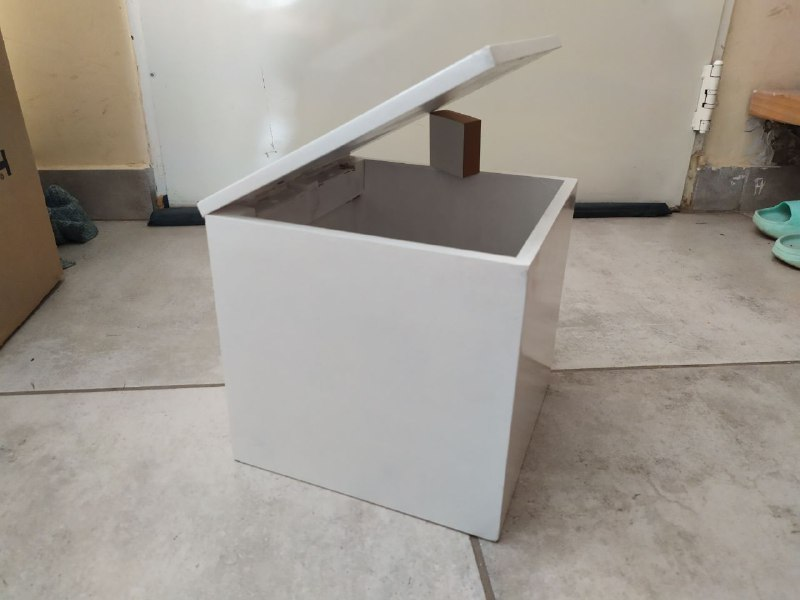
\includegraphics[width=.9\linewidth]{../../images/cuboFisico.png}
\caption{\label{fig:cuboFisico}Carcasa del SATDAC}
\end{figure}

\begin{figure}[htbp]
\centering
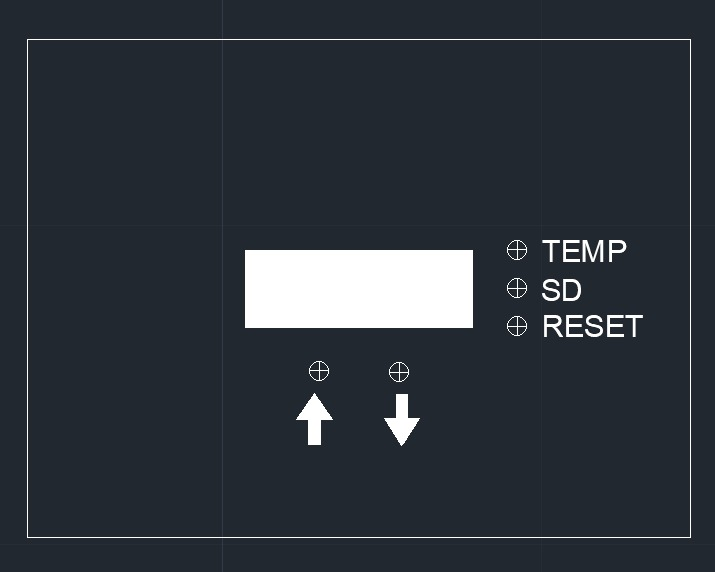
\includegraphics[width=.9\linewidth]{../../images/estacionFisico.png}
\caption{\label{fig:estacionFisico}Carcasa de la ERDYTC}
\end{figure}

\subsection{Diagrama en bloques:}
\label{sec:orgea1461d}
En la Fig. \ref{fig:diagramaBloques} se puede visualizar el diagrama en bloques completo de ambos sistemas interconectados.

\begin{figure}[htbp]
\centering
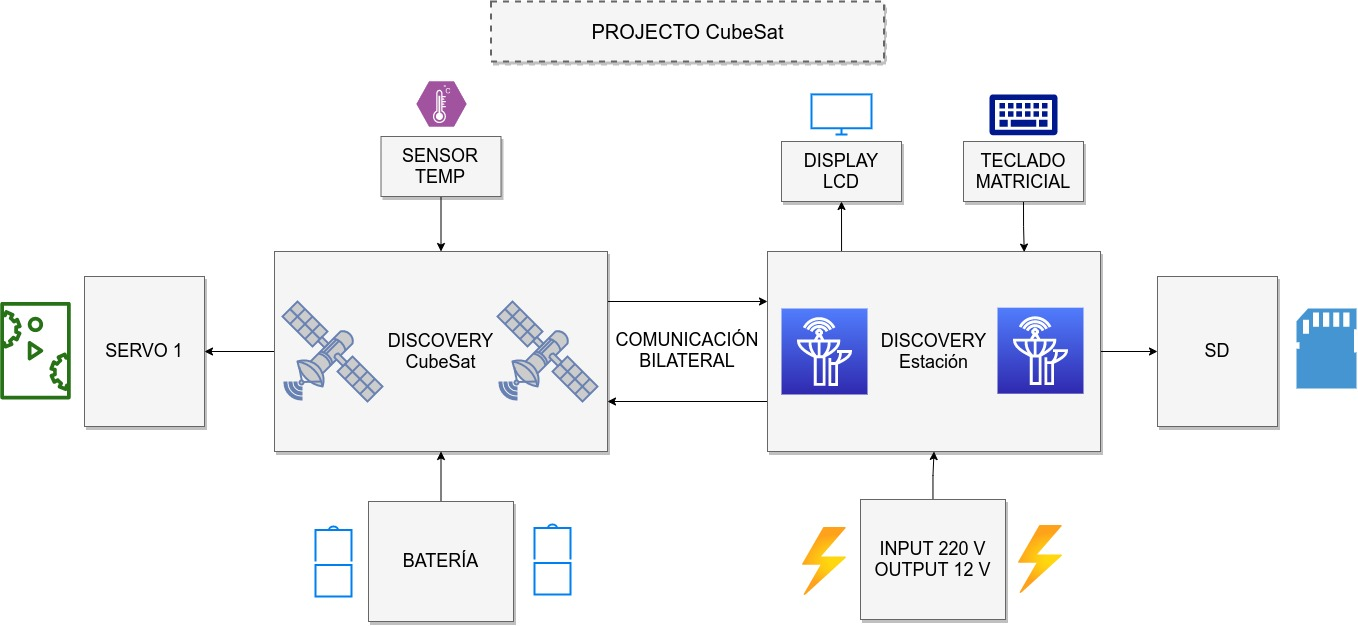
\includegraphics[width=.9\linewidth]{../../images/diagramaBloques.jpg}
\caption{\label{fig:diagramaBloques}Diagrama en bloques de los sistemas}
\end{figure}

En el mismo se puede observar de forma gráfica las distintas conexiones y funciones de los sistemas descritos en este documento. Se observa que el SATDAC posee como alimentación una batería de 3.7 [V], y la ERDYTC se alimenta a partir de la RED. Además, se denotan los diferentes periféricos utilizados en ambos sistemas.
\subsection{Descripción del circuito ERDYTC:}
\label{sec:org7083e39}
En la Fig. \ref{fig:estacionEsquematico} se puede observar el circuito esquemático que representa la ERDYTC.

\begin{figure}[htbp]
\centering
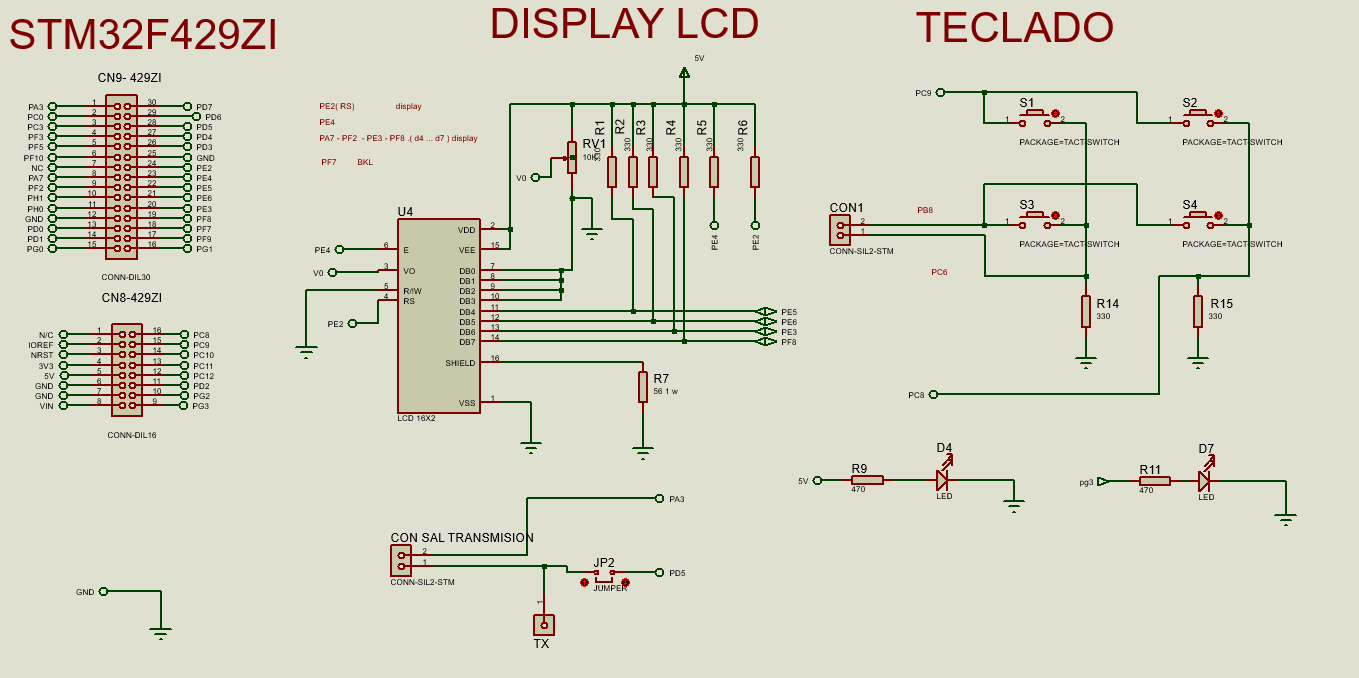
\includegraphics[width=.9\linewidth]{../../images/estacionEsquematico.png}
\caption{\label{fig:estacionEsquematico}Circuito esquemático de la ERDYTC}
\end{figure}

En el mismo se describe el conexionado del sistema:

\begin{itemize}
\item Se utilizaron los conectores CN8 y CN9 de la STM32F429ZI para realizar todas las conexiones a través de un poncho.
\item La conexión del display LCD se realizó con resistencias de pull-up a 5 voltios, y las conexiones a los pines de la STM se dan todas en el conector CN9.
\item La conexión de los pulsadores se da en forma matricial.
\end{itemize}

\begin{figure}[htbp]
\centering
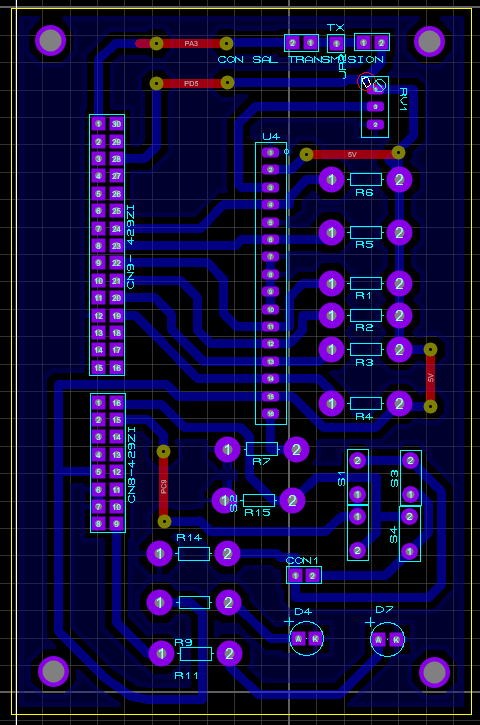
\includegraphics[width=.9\linewidth]{../../images/estacionPCB.png}
\caption{\label{fig:estacionPCB}ERTDYC PCB}
\end{figure}

Luego, en la Fig. \ref{fig:estacionPCB} se puede observar el circuito impreso o PCB de la ERDYTC. En el mismo se nota claramente que se utilizó el conector de Arduino de la STM para realizar el poncho con la placa.

\begin{figure}[htbp]
\centering
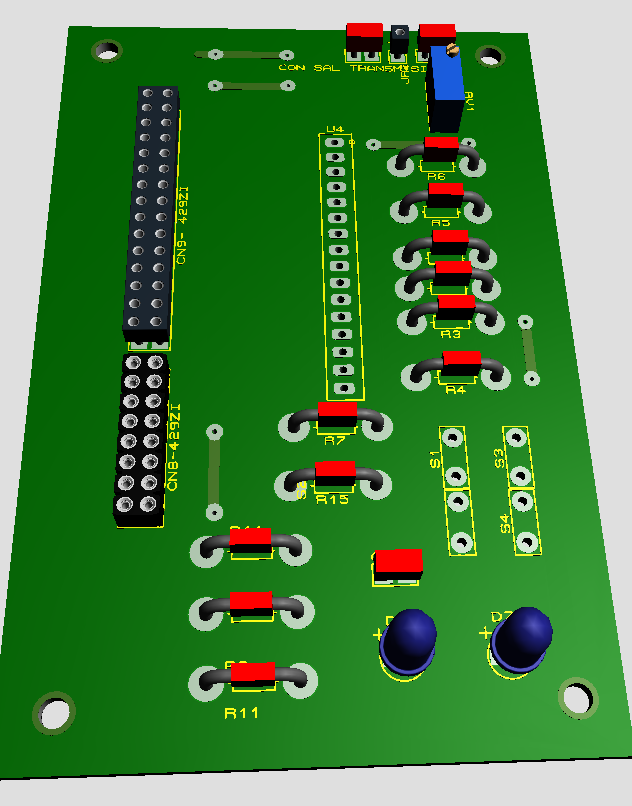
\includegraphics[width=.9\linewidth]{../../images/estacion3D.png}
\caption{\label{fig:estacion3D}Render 3D del PCD de la ERDYTC}
\end{figure}

Finalmente, en la Fig. \ref{fig:estacion3D} se puede observar el PCB físico de la ERDYTC.
\subsection{Descripción del circuito SATDAT:}
\label{sec:org96f9a21}
En la Fig. \ref{fig:cuboEsquematico} se puede observar el diagrama esquemático del SATDAC.

\begin{figure}[htbp]
\centering
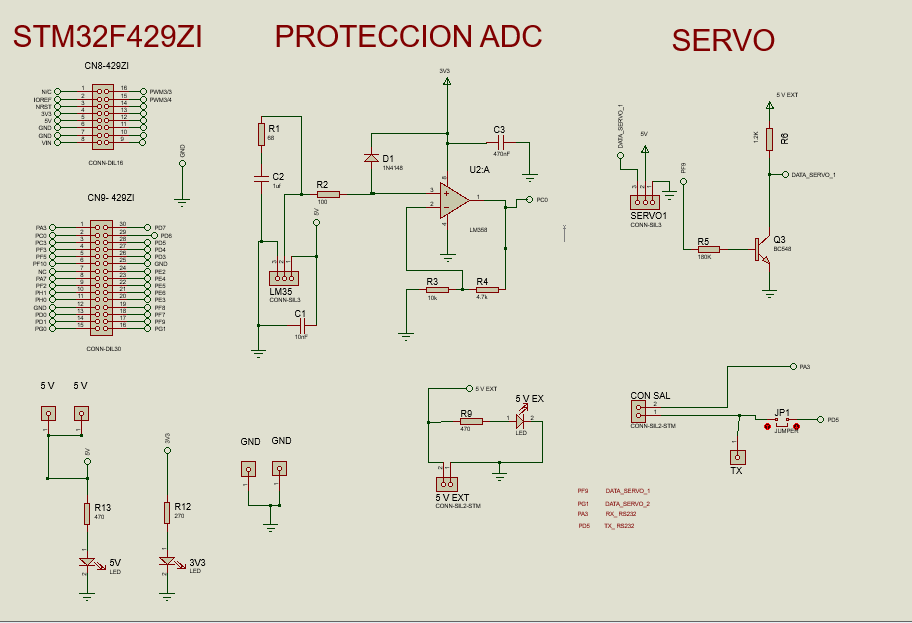
\includegraphics[width=.9\linewidth]{../../images/cuboEsquematico.png}
\caption{\label{fig:cuboEsquematico}Esquemático del SATDAC}
\end{figure}

En el mismo se puede ver el conexionado del sistema:

\begin{itemize}
\item Se utilizaron los conectores CN8 y CN9 de la STM para realizar el poncho.
\item Se utilizó un circuito amplificador de protección para el conexionado del sensor de temperatura LM35.
\end{itemize}

Los puertos UART usados tanto en el SATDA como ERDYTC fueron el PA2 y PA3 respectivamente, y se corresponden con el UART2 en el sistema.

\begin{figure}[htbp]
\centering
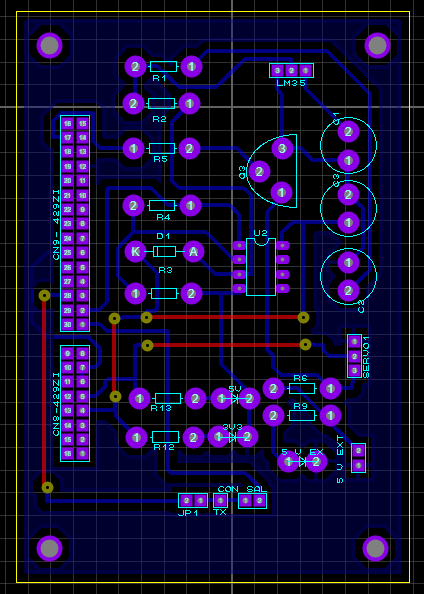
\includegraphics[width=.9\linewidth]{../../images/cuboPCB.png}
\caption{\label{fig:cuboPCB}SATDAC PCB}
\end{figure}

\begin{figure}[htbp]
\centering
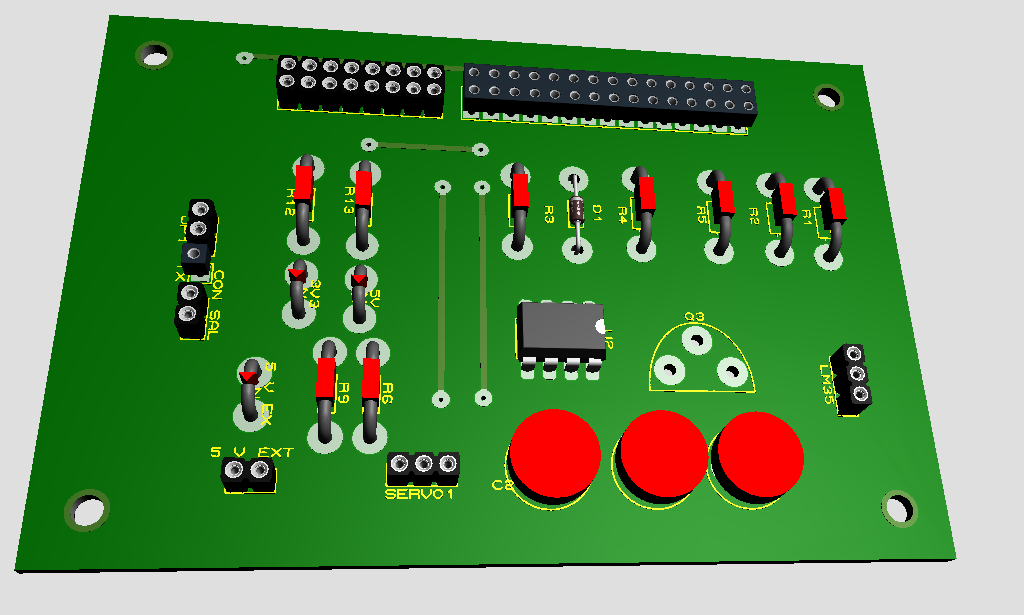
\includegraphics[width=.9\linewidth]{../../images/cubo3D.png}
\caption{\label{fig:cubo3D}SATDAC 3D}
\end{figure}

Luego en la Fig. \ref{fig:cuboPCB} se puede observar el PCB del SATDAC, y en la Fig. \ref{fig:cubo3D} el modelo 3D del mismo.

\section{Software:}
\label{sec:org76ebab6}
\subsection{Código fuente:}
\label{sec:org257aa8a}
La descripción completa de todo el software se puede visualizar en el siguiente enlace: \url{https://github.com/AugustoRiedinger/tecDig2\_project/tree/master/code}.

En el mismo, también se pueden descargar y contribuir a todos los archivos tanto del software como del proyecto en general.

En la carpeta \emph{code} se puede encontrar y editar el código fuente que se carga en ambos sistemas. Notar que el archivo \emph{hardware.h} describe los pines utilizados para los dos sistemas; el mismo se puede editar fácilmente y a conveniencia que cambiará todas las funciones donde sea utilizado.
\subsection{Lenguaje:}
\label{sec:orgcd06b6a}
El lenguaje utilizo en todas las librerías creadas y el código fuente es C, junto con funciones específicas desarrolladas por ST.

C es un lenguaje de programación de propósito general originalmente desarrollado por Dennis Ritchie entre 1969 y 1972 en los Laboratorios Bell,​ como evolución del anterior lenguaje B, a su vez basado en BCPL.

Al igual que B, es un lenguaje orientado a la implementación de sistemas operativos, concretamente Unix. C es apreciado por la eficiencia del código que produce y es el lenguaje de programación más popular para crear softwares de sistemas y aplicaciones.

Se trata de un lenguaje de tipos de datos estáticos, débilmente tipado, de medio nivel, que dispone de las estructuras típicas de los lenguajes de alto nivel pero, a su vez, dispone de construcciones del lenguaje que permiten un control a bajo nivel. Los compiladores suelen ofrecer extensiones al lenguaje que posibilitan mezclar código en ensamblador con código C o acceder directamente a memoria o dispositivos periféricos.

\subsection{Entorno de desarrollo:}
\label{sec:orgd6c0ea7}
Para editar los archivos principalmente se utilizó el software Doom Emacs; luego para debuggear se utilizó Atollic TRUEStudio.

Los programas utilizados tanto para editar como para debuggear son a elección, pero los autores solamente testearon en los mencionados.
\end{document}
